\documentclass[11pt]{beamer}
\usetheme{CambridgeUS}
\usepackage[utf8]{inputenc}
\usepackage[french]{babel}
\usepackage[T1]{fontenc}
\usepackage{amsmath}
\usepackage{amsfonts}
\usepackage{amssymb}
\usepackage{graphicx}
\author{Dr OM}
\title{Analyse Factorielle des Correspondances (AFC)}
%\setbeamercovered{transparent} 
%\setbeamertemplate{navigation symbols}{} 
%\logo{} 
\institute{LMI-SFA-UNA} 
%\date{} 
%\subject{} 
\begin{document}

\begin{frame}
\titlepage
\end{frame}

\begin{frame}
\tableofcontents
\end{frame}
%%%%%%%%%%%%%%%%%%%%%%%%%%%%%%%%%%
\section{Test Khi2}
%\subsection{Problématique}
\begin{frame}{Structure de base des données}
Objective mesurer des liaisons entre deux variables qualitatives :\textcolor{blue}{Khi-deux}\\
exemple : 
Il s’agit de tester l’indépendance de deux variables qualitatives.
Y a-t-il indépendance entre :


\begin{itemize}
\item la catégorie socioprofessionnelle et le vote à l’élection
présidentielle ?
\item  le niveau d’études et les journaux lus ?
\end{itemize}

\begin{figure}
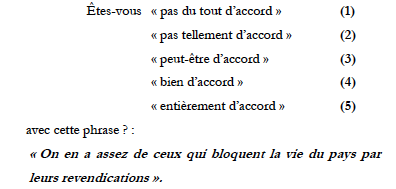
\includegraphics[scale=0.6]{Exemple.png}  
\end{figure}
\end{frame}

\begin{frame}{}
\begin{figure}
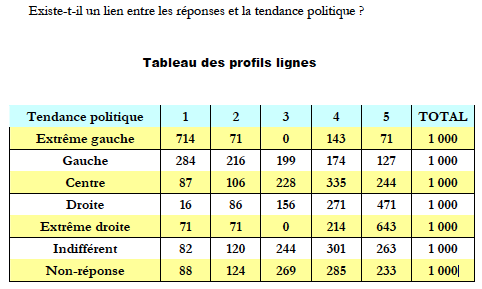
\includegraphics[scale=0.6]{Exemple2.png}  
\end{figure}
\end{frame}

\subsection{Le test du Khi2}




\begin{frame}{Le tableau de contingence}
\begin{figure}
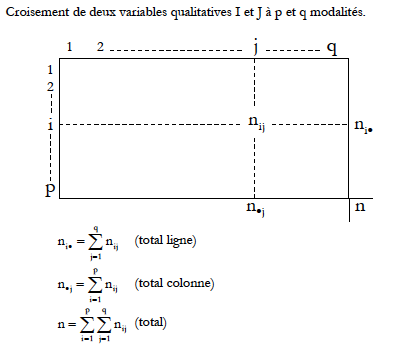
\includegraphics[scale=0.6]{Exemple3.png}  
\end{figure}
\end{frame}

\begin{frame}{Notations : tableau de contingence : N}
Croisement de deux variables qualitatives à p et q modalités

\begin{figure}
\includegraphics[scale=0.7]{exemple8.png}  
\end{figure}
\end{frame}

\begin{frame}{Profils lignes - profils-colonnes - profils
marginaux}
\begin{figure}
\includegraphics[scale=0.7]{exemple9.png}  
\end{figure}
\end{frame}



%\begin{frame}{}
%
%\begin{figure}
%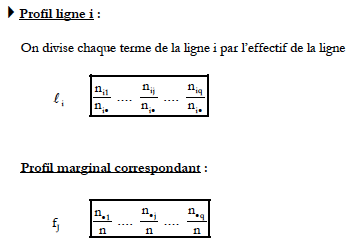
\includegraphics[scale=0.7]{Exemple4.png}  
%\end{figure}
%
%%\textcolor{blue}{Si les deux variables qualitatives I et J étaient indépendantes, les profils lignes seraient tous identiques, et donc identiques au profil marginal correspondant.}
%\end{frame}


\begin{frame}{Profils lignes - profils-colonnes - profils
marginaux}

\textcolor{blue}{Si les deux variables qualitatives I et J étaient indépendantes, les profils lignes seraient tous identiques, et donc identiques au profil marginal
correspondant.}

$$Independance \Rightarrow \frac{n_{ij}}{n_{i \bullet}}=\frac{n_{\bullet j}}{n} \Rightarrow n_{ij}=\frac{n_{\bullet j}*n_{i \bullet}}{n}$$

\end{frame}


\begin{frame}{Profils lignes - profils-colonnes - profils
marginaux}

\begin{itemize}
\item  On pouvait établir la relation précédente en raisonnant sur les profils colonnes.
\item 

\begin{figure}
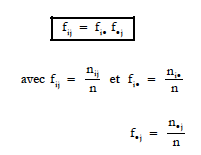
\includegraphics[scale=0.7]{Exemple5.png}  
\end{figure}
\end{itemize}

\textcolor{blue}{Elle exprime clairement que dans le cas de l’indépendance le tableau de contingence est entièrement déterminé par ses marges
}
\end{frame}

\begin{frame}{Définition du Khi-deux}
\begin{itemize}
\item Pour chaque case, on peut donc calculer le nombre de cas attendus \textcolor{blue}{(sous hypothèse d’indépendance)}
$n_{ij}=\frac{n_{\bullet j}*n_{i \bullet}}{n} $

\item On peut comparer les nombres de cas attendus $E_{ij}$ aux nombres observés.

\begin{figure}
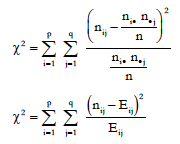
\includegraphics[scale=0.8]{Exemple6.png}  
\end{figure}
\end{itemize}
\end{frame}
%%%%%%%%%%%%%%%%%%%%


\begin{frame}{}

Si les deux variables sont réellement indépendantes, cette expression suit une distribution du Khi-deux avec un nombre de degrés de liberté égal
à : $(p -1) (q -1)$\\

Dans une table on lit $\chi_{\alpha,k}^2$ valeur ayant une probabilité
$\alpha$ d’être dépassée


pour une distribution du khi-deux avec $k = (p-1) (q -1)$
degrés de liberté.

\begin{enumerate}
\item Si $\chi^2\leq \chi_{\alpha,k}^2$  On accepte $H_o$ : independance 
\item  Si $\chi^2 > \chi_{\alpha,k}^2$  On rejette $H_o$ : independance 
\end{enumerate}

\end{frame}
%%%%%%%%%%%%%%%%%%%%%%%%%%%%%%%
\begin{frame}{Pratique sous logiciel statistique}

\begin{itemize}
\item  Calcul du $\chi^2$ associé au tableau de contingence noté $\chi^2_{obs}$.

\item Probabilité pour une v.a. suivant une loi du khi-deux à
$(p -1) (q -1)$ d.d.l. de dépasser $\chi^2_{obs}$.

\begin{figure}
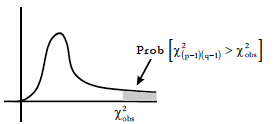
\includegraphics[scale=0.8]{exemple7.png}  
\end{figure}

\end{itemize}


\textcolor{blue}{Si cette probabilité est faible (en général < 5 \%), on rejette l’hypothèse d’indépendance entre les deux variables qualitatives.}


\end{frame}


\section{L’analyse des correspondances simples}
\begin{frame}{AFC}

\begin{itemize}
\item  Répartition des habitants d'Abidjan selon leur lieu
d’habitation  et leur C.S.P.

\begin{itemize}
\item Certains quartiers sont-ils proches ?
\item  au sens même répartition des C.S.P. ?
\item Certaines C.S.P. sont-telles proches ?
\item Certaines C.S.P. sont-elles plus souvent associées à
certains quartiers ?
\end{itemize}
\end{itemize}

\textcolor{blue}{L’analyse des correspondances traite des tableaux de contingence.}
\end{frame}
%%%%%%%%%%%%%%%%%%%%%%%%%%%%%%%
\subsection{Notations et présentation}
%%%%%%%%%%%%%%%%%%%%%%%%%%%%%%%%%

\begin{frame}{Représentation des profils lignes}
\begin{itemize}
\item Les profils lignes sont considérés comme des individus.\\
\item Les p profils-lignes forment un nuage de p points dans $R^q$\\

\item A chaque profil-ligne est associé un poids égal à sa fréquence marginale profil ligne poids
$f_{i \bullet}$.
\end{itemize}
On note $N(I)$ le nuage de points formé des profils-lignes pondérés :
$( l_i; f_{i \bullet})$

Le centre de gravité g est défini par : $$ g_l=\sum_{i=1}^p f_{i \bullet}l_i$$

La jième coordonnée de $g_l$ vaut $f_{\bullet j}$

Donc \textcolor{blue}{$g_l$ = profil marginal de la variable J (à q modalités) $g_l=f_J$}

\end{frame}
%%%%%%%%%%%%%%%%%%%%%%%%
\begin{frame}{Représentation des profils lignes}
\begin{figure}
\includegraphics[scale=0.7]{exemple10.png}  
\end{figure}
\end{frame}
%%%%%%%%%%%%%%%%%%%%%%%%%%
\begin{frame}{}
\begin{figure}
\includegraphics[scale=0.5]{exemple11.png}  
\end{figure}
\end{frame}

%%%%%%%%%%%%%%%%%%%%%%%%%%%%
\begin{frame}{Métrique du $\chi 2$}

\begin{itemize}
\item Pour les profils lignes :\\

$$d^2_{\chi^2}(l_i,l_i')=\sum_{j=1}^{q}\frac{n}{n_{\bullet j}}(\frac{n_{ij}}{n_{i \bullet}}-\frac{n_{i'j}}{n_{i' \bullet}})^2  $$

\begin{itemize}
\item Donne un poids important aux différences portant sur les
petits pourcentages.
\item  Vérifie le principe d’équivalence distributionnelle : si deux
colonnes ont le même profil, on les réunit en une seule
d’effectif somme sans modifier les distances entre profilslignes.
\end{itemize}

\item Pour les profils-colonnes :

$$d^2_{\chi^2}(c_j,c_j')=\sum_{j=1}^{q}\frac{n}{n_{i \bullet }}(\frac{n_{ij}}{n_{\bullet j}}-\frac{n_{ij'}}{n_{ \bullet j'}})^2  $$       
       
\end{itemize}
\end{frame}
%%%%%%%%%%%%%%%%%%%%%%%%%%%%%
\begin{frame}{Inertie du nuage N(I)}
$I_{N(I)}$  l’inertie du nuage$ N(I)$ calculée par rapport
au centre de gravité $f_J$ vaut $$\frac{\chi^2}{N}$$

où $\chi^2=$ Khi-deux associé au tableau de contingence étudié.\\

\textcolor{blue}{On obtient le même résultat pour l’inertie du nuage N(J).}

\end{frame}
\subsection{ACP du nuage des profils lignes-profils colonnes }
\begin{frame}{l’A.C.P. du nuage des profils-lignes :}
\begin{itemize}

\item Les profils-lignes jouent le rôle d’individus ; ils sont
affectés des poids $f_{i\bullet}$
\item La métrique utilisée pour le calcul des distances entre
individus est la métrique du khi-deux

\item Le premier axe principal du nuage des profils-lignes est la droite passant le plus près possible de l'ensemble des points
de N(I).
\end{itemize}
\end{frame}

\begin{frame}{l’A.C.P. du nuage des profils-lignes }
\begin{figure}
\includegraphics[scale=0.8]{exemple12.png}  
\end{figure}
\end{frame}
%%%%%%%%%%%%%%%%%%%%%%%%%
\begin{frame}{’A.C.P. du nuage des profils-colonnes}
\begin{figure}
\includegraphics[scale=0.6]{exemple13.png}  
\end{figure}
\end{frame}
\subsection{Lien entre les deux analyses }

\begin{frame}{Formules de transition}

En notant $b_j$ et $a_i$ les $j^{ème}$ et $i^{ème}$ coordonnées des composantes principales \textit{b} et \textit{a} associées à la même valeur propre $\lambda$ : 

$$ \sqrt{\lambda}b_i=\sum_{i=1}^p\frac{n_{ij}}{n_{\bullet j}}  $$

$$ \sqrt{\lambda}a_i=\sum_{j=1}^q\frac{n_{ij}}{n_{i \bullet }}  $$


\textcolor{blue}{À $\lambda$ près, la coordonnée d’une modalité i d’une variable est la moyenne des coordonnées des catégories de l’autre variable pondérées par les fréquences conditionnelles du profil de i.}
\end{frame}

\subsection{Représentation de l'A.F.C.}

\begin{frame}{Les modalités de la variable I sont représentées en tant qu’individus (profils-lignes) de l’A.C.P. des profils-lignes.}

\begin{figure}
\includegraphics[scale=0.6]{exemple14.png}  
\end{figure}

\end{frame}

\begin{frame}{Les modalités de la variable I sont représentées en tant qu’individus (profils-lignes) de l’A.C.P. des profils-lignes.}

\begin{figure}
\includegraphics[scale=0.6]{exemple15.png}  
\end{figure}

\end{frame}

\begin{frame}{Abandon du principe barycentrique}

Les modalités de chaque ensemble sont représentées par les :

$$a^k_i,  i=1, \ldots, p$$

$$b^k_j ,  j=1, \ldots, q $$

Cette représentation permet de déterminer les proximités entre
certains éléments de I et certains éléments de J (compte tenu de la
qualité de la représentation).

\end{frame}

\subsection{Aides à l’interprétation : identiques à celles de l’A.C.P.}
\begin{frame}{Contributions}
\begin{figure}
\includegraphics[scale=0.6]{exemple16.png}  
\end{figure}
\end{frame}

\begin{frame}{Cosinus carrés}
\begin{figure}
\includegraphics[scale=0.6]{exemple17.png}  
\end{figure}

\end{frame}

\begin{frame}{Aspects pratiques de l’interprétation}

\begin{itemize}
\item L’interprétation peut se faire à partir des représentations graphiques (en s’assurant de la qualité de représentation de chaque modalité à
l’aide des cos2).
\item Quand le nombre de modalités est élevé, il est conseillé d’éditer d’abord le graphique des profils-lignes, puis celui des profilscolonnes, enfin la représentation simultanée.

\item Les profils ayant des poids différents la lecture de leurs
contributions à l’inertie de chaque axe s’avère très utile.

\item On peut repérer les profils dont la contribution est supérieure au poids
\end{itemize}
\end{frame}

\section{Cas pratique}
\begin{frame}{}

\end{frame}


\end{document}